\chapter{Activités confiées pendant le stage}
Pendant mon stage j'ai participé à beaucoup de fiches différentes, il serait long et ennuyeux de les détailler toutes sachant que je participai à entre 1 et 4 fiches par semaine. Je présenterai dans les grandes lignes les fonctionnalités majeure auxquelles j'ai participé. 

\section{Développements sur le code de production}
Parmi les activité qui m'ont été confiées, j'ai participé à la réalisation de fiches blanches (cf. \ref{agile:fiches} \pageref{agile:fiches}). Ce code est appelé ``code de production'' car il couvre les besoins fonctionnels exprimés par le client XP. La première étape dans le travail sur une fiche est de préciser le périmètre fonctionnel avec le client XP. Ceci permet aux développeurs de connaitre son besoin précis. Ensuite, dans la mesure du possible, on crée les tests unitaires qui permettront de savoir si la fonctionalité est opérationnelle. Les membres du binôme peuvent prendre le clavier au moment où ils le souhaitent et proposer leurs idées. Chaque direction prise et ainsi refléchie et validée par chaque memebre du binôme.

\subsection{Observations}

\subparagraph*{}
Au début de mon stage, la première fonctionalité sur laquelle j'ai travaillé fut des observations. Dans le produit, le observations sont des stéréotypes\footnote{stéréotypes au sens UML} attachés à des opérations de classes du modèle de test. Les observations sont déclenchées par des triggers\footnote{Evènement déclencheur} selon une précondition décrite dans le langage OCL(cf. lexique \ref{lexique:OCL} p.\pageref{lexique:OCL}). Dans les modeleurs, à l'export, ce stéréotype est reconnu et intégré au modèle propre à Test Designer. Les observations font office de ``points de contrôle '' permettant de vérifier que le système sous test réagit correctement.

\subparagraph*{}
Les observations sont introduites dans les deux modeleurs principaux de façon différente. Dans RSM, les stéréotypes et la gestion des triggers spécifiques à SMARTESTING proviennent d'un profil personnalisé. L'utilisation des profils dans le modeleur Together ont été l'occasion d'une autre fiche à laquelle j'ai contribué. Cependant mon binôme et moi-même nous somme rendu compte, après avoir passé 4 points de vélocité sur cette fiche cotée à 2, que c'était plus compliqué que nous l'imaginions. Nous avons alors suspendu la fiche en attente de conseils d'OBEO\footnote{OBEO est une société de conseil experte dans le domaine de la modélisation EMF/GMF sous Eclipse}. Finalement la après leur réponse, nous avons dù Rollback(cf. lexique \ref{lexique:rollback} p.\pageref{lexique:rollback}) notre travail. La solution adaptée finalement fut d'utiliser le code péexistant. C'est à dire utiliser des propriétés ``Custom''(cf. figure \ref{figure:obsTriggerTG} p.\pageref{figure:obsTriggerTG}) pour gérer les triggers dans Together. Ces triggers servent à déterminer les opérations que l'on souhaite observer. Une fois définies dans le modèle UML et après export, les observations sont visibles dans Test Designer (cf. figure\ref{figure:obsTD} p.\pageref{figure:obsTD}).

\begin{figure}[!ht]
\centering
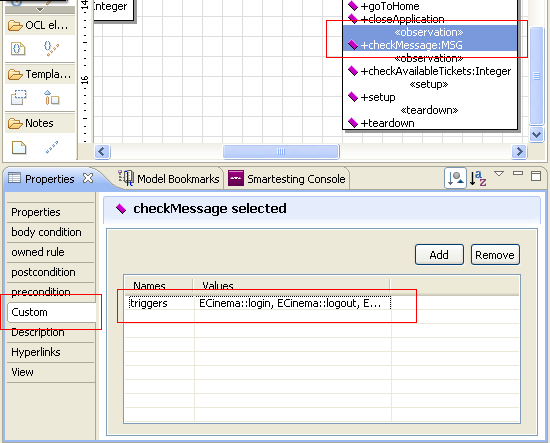
\includegraphics[scale=0.5]{Illustrations/Observation_Trigger_Together.png}
\caption{Intégration des observations dans Together}
\label{figure:obsTriggerTG}
\end{figure}

\begin{figure}[!ht]
\centering
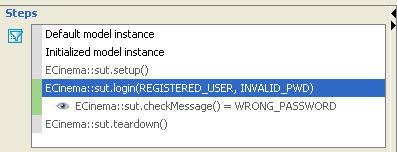
\includegraphics[scale=0.5]{Illustrations/Observation.png}
\caption{Intégration des observations dans Test Designer}
\label{figure:obsTD}
\end{figure}

\subsection{Descriptions}

\subparagraph*{}
Dans test Designer, plusieurs élements ont besoin d'être décrits afin d'être exploitable à la publication par exemple dans la publication HTML, HP Mercury Quality Center ou encore dans Rational Quality Manager. A l'origine les descriptions qui étaient dejà implémentées etaient puibliées en texte brut. Après un court spike (cf. lexique \ref{lexique:spike} p.\pageref{lexique:spike}) nous nous sommes aperçu que plusieurs publishers supportaient des balises HTML. Il était egalement possible de mettre du texte en forme en amont dans les modeleurs (cf. tableau \ref{tableau:compatDescHTML} p. \pageref{tableau:compatDescHTML}). Néanmoins certaines version de modeleurs n'ont pas les mêmes standards de mise en forme des descriptions. Ainsi il a fallu passer par une étape intermédiaire pour unifier les descriptions dans un format spécifique interne. Il est par exemple necessaire d'enlever certaines balises en trop ou encore de convertir des balises en d'autres plus globalement supportées. Nous avons choisi d'utiliser le format XHTML avec l'aide de la bibliothèque JTidy (cf \ref{figure:descXHTMLPublisher} p. \pageref{figure:descXHTMLPublisher}). Les descriptions obtenues sont ensuite ``rendues'' pour être affichées ainsi qu'on le souhaite dans les différents publishers.

\begin{table}[!ht]
\caption{\label{tableau:compatDescHTML}Compatibilité HTML des modeleurs et publishers}
\begin{tabular}{|l|l|l|}
  \hline
  Type & Nom & Balises supportées (simplifié) \\
  \hline
  \hline
  \multirow{4}{*}{Modeleurs} & Together 2007 & HTML <b><i><u> \\
    & RSM 7.0.0.x & texte brut\\
    & RSM 7.0.5.x & HTML <b><i><u> + centrer + paragraphes\\ 
   & RSM 7.5 &  HTML <b><i><u>+ centrer + paragraphes + autres\\ \hline
  \multirow{3}{*}{Publishers} & HTML &  \\
    & Quality Center & texte brut et HTML <b><i><u> \\
    & Specification (pdf) & <strong><em><ins>  \\
    & Prototype RQM &  HTML <b><i><u> \\ \hline
\end{tabular}
\end{table}


\begin{figure}[!ht]
\centering
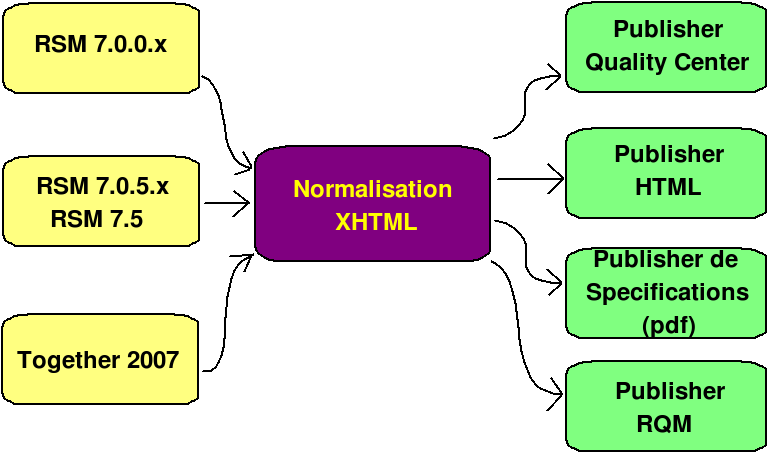
\includegraphics[scale=0.5]{Illustrations/bigDescSchema.png}
\caption{Passage des descriptions des modeleurs à leur publication}
\label{figure:descXHTMLPublisher}
\end{figure}

\subsection{Test Suites}
Les suites de test permettent d'avoir une unité structurante pour tout un ensemble de test à partir des modeleurs. Elles définissent le périmètre des tests. Auparavant, une suite de test était considérée implicitement dans le modèle. Les différents packages\footnote{Equivalent d'un dossier pour stocker des ressources dans Eclipse dans le cadre de la modélisation} contenant des informations relatives aux suites etaient analysés puis elles étaient personalisées (filtre) dans le Target Manager. 

\subparagraph*{}
En fin du dernier jalon, guidé par des besoins de pouvoir remonter des informations des suites jusque là difficilement accessibles. Le client XP après plusieurs discussions avec l'équipe a décidé qu'il fallait externaliser les suites de test dans des fichiers de type texte. Cette modification de la structure des suite doit permettre d'être une étape de base pour rendre la solution Smartesting ``verticale'' afin de pouvoir par exemple s'intégrer à SAP. La solution choisie a été d'utiliser un fichier texte écrit dans un langage facile à écrire et à comprendre : Yaml\footnote{``YAML Ain't Markup Language''; il s'agit d'un langage dédié à la serialisation (cf. lexique \ref{lexique:serialisation} p.\pageref{lexique:serialisation})}. Yaml est dit ``user friendly'' facile à lire et à comprendre pour un utilisateur.

\begin{figure}[!ht]
\centering
\ttfamily{
\small{
\begin{verbatim}
# un commentaire et un tableau
users:
  - Toto
  - Titi

# utilisation de booléens
vrai: true
faux: false

# tableaux associatifs multidimensionnels
foo:
  toto:  gentil
  titi:  mechant
\end{verbatim}
}
}
\caption{Exemple de fichier YAML}
\label{figure:exYaml}
\end{figure}

\begin{figure}[!ht]
\centering
\ttfamily{
\small{
\begin{verbatim}
--- !TestSuite
identifier: 4d517188-80af-4255-9405-abc367dcb5a7
initialModelInstance: initial_model_instance
version: "1.0"
\end{verbatim}
}
}
\caption{Exemple de fichier YAML pour les TestSuite}
\label{figure:exTestSuite}
\end{figure}

\subparagraph*{}
Malgré son apparence simple, l'extraction des suite de test a été difficile. Tout d'abord l'équipe ayant peu de conaissances dans Eclipse sur certains domaines relatifs à cette fonctionalité, il a fallu un certain temps d'adaptation. Les différences entre les différents modeleurs ont rendu la tâche encore plus difficile.



\section{Correction de bugs}
La correction de bugs fait partie du travail des développeurs même si ce n'est pas forcément agréable. Toutefois les tests, la validation, l'intégration continue et les itérations courtes rendent la détection de bugs très rapide. La plupart des bugs sont en général détectés et corrigés avant la livraison en fin de semaine. Dans l'équipe on considère qu'il existe deux types de bugs. Les bugs client sont des bugs qui ont été remontés par les utilisateurs finaux après une release officielle. Les autres bugs qui sont détectés pendant l'itération ou après des releases mineures ne sont pas considérés comme des bugs client. Cette distinction est importante car, en adoptant la pratique ``No Bugs'' l'équipe s'engage à livrer un produit de qualité avec un minimum d'anomalies. L'équipe R\&D s'est fixée comme obtectif pour l'année d'avoir moins de 40 bugs client. Cet engagement influe sur la prime de l'équipe.

\section{Documentation}


\section{Validation}
La validation joue un rôle important lors de l'itération. Une partie de la validation est réalisée en permanence par les serveurs d'intégration continue. Une autre partie (en général, l'utilisation via l'interface homme-machine) ne peut être réalisée que par des personnes qui n'ont pas participé au développement de la fonctionnalité. Cela permet d'avoir une idée plus objective des manipulations à effectuer pour tester la fonctionnalité. Au cours de la semaine la validation est la tâche exclusive de Batman. Il valide une fiche dès qu'elle a été mise ``À valider'' afin d'avoir le retour le plus rapide sur la fonctionnalité. Lors de la validation, on fait très souvent appel au client XP pour vérifier que la fonctionnalité correspond bien aux besoin énoncés. À la fin de l'itération, lorsque toutes les fiche sont terminées et validées, l'équipe commence une validation de l'ensemble des fiches de l'itération. Lorsque toute l'équipe est satisfaite (les bugs éventuels corrigés, documentation relue ...) la livraison peut avoir lieu.

\section{Amélioration du code existant (refactoring)}
TODO : utilité ,exemple, 

\section{Prototypes}

\section{Administration système}
Sur une courte période j'ai effectué des t\^aches d'administration système. En particulier au moment de l'intégration des Google Apps dans le fonctionnement de Smartesting. La necessité de partager des calendriers et de pouvoir y accéder via des plateformes mobiles a amené Smartesting à envisager d'utiliser Google Apps. Ainsi, en binôme avec Olivier, nous avons appréhendé le panneau d'administration ainsi que les différents services utilisables. Chaque calendrier donne la possibilité d'être exporté, ainsi nous avons pu réaliser une routine de backup\footnote{sauvegarde automatique}.

\section{Réunions et Meeting corporate}

TODO : definition, utilité, ma participation ...

\subsection{Visite de BNP Paribas}
Mes impressions, les decisions, Smart et BNP ...

\subsection{Amélioration du process, évolution du fonctionnement de l'équipe}
J'ai été ammené à l'occasion de retrospectives ou de réunions à réfléchir sur le processus de développement au sein de l'équipe. L'équipe de R\&D est très concernée par l'amélioration du processus et toute pratique peut être remise en cause si elle ne convient pas a l'équipe. Chaque décision quelle qu'elle soit doit être approuvée par toute l'équipe avant d'être prise. Je parlerai plus en détail à travers d'exemple du type de décisions qui sont prises sur ce sujet.

\subsection{Evaluation}



Tableau des évolution des pratiques XP
\begin{table}[!ht]
	\caption{\label{tableau:evolPratXP}Evolution des pratiques XP au cours du stage}
	\begin{tabular}{|l|c|c|}
		\hline
		Pratique & Début du stage & Fin du stage\\
		\hline
		Pair programming & \tick & \tick \\
		Itération & 2 semaines & 1 semaine \\
		Intégration continue & \tick & \tick \\
		Niko Niko & \tick & \badtick \\
		Lecture & \tick & \badtick \\
		Point perso & hebdomadaire & nouvelles experimentations\\
		Pomodoro & \badtick & \tick \\
		Test driven development & \tick & \tick \\
		``Done done'' & théorique & adopté et normalisé\\
		``No Bugs'' & imprécis & engagement \\
		Slack Time & \badtick & adopté et normalisé\\
		Rétrospective & 1 à 2h le lundi matin & Timeboxée et juste après la livraison\\
		Point technique & assez réguliers & moins nombreux\\
		Veilleur & \tick & Robin cumule son rôle\\
		Batman/Robin & \badtick & \tick \\
		\hline
	\end{tabular}
\end{table}


TODO : Decisions lors de retrospectives, Iteration 1 semaine, Slack, reduction de vélocité, Done-done, rédaction(et simplification) des standards, Objectifs R\& D, ...